\chapter{Folding and Tracing Constructions}
\begin{quote} 
We don't even know if Foldspace introduces us to one universe or
many\dots

\hfill---Frank Herbert
\end{quote}

\section{Constructions}

While origami as an art form is quite ancient, folding and tracing constructions
in mathematics are relatively new. The earliest mathematical
discussion of folding and tracing constructions that I know of appears in
T.\ Sundara Row's book \textit{Geometric Exercises in Paper Folding},
\cite{row}, first published near the end of the Nineteenth Century. In
the Twentieth Century it was shown that every construction that is
possible with a compass and straightedge can be done with
folding and tracing. Moreover, there are constructions that are possible via
folding and tracing that are \textit{impossible} with compass and straightedge
alone. This may seem strange as you can draw a circle with a compass,
yet this seems impossible to do via paper-folding. We will address
this issue in due time. Let's get down to business---here are the
rules of folding and tracing constructions:


\subsubsection{Rules for Folding and Tracing Constructions}
\begin{enumerate}
\item You may only use folds, a marker, and semi-transparent paper.
\item Points can only be placed in two ways:
\begin{enumerate}
\item As the intersection of two lines. 
\item By marking ``through'' folded paper onto a previously placed
  point. Think of this as when the ink from a permanent marker
  ``bleeds'' through the paper.
\end{enumerate}
\item Lines can only be obtained in three ways:
\begin{enumerate}
\item By joining two points---either with a drawn line or a fold.
\item As a crease created by a fold. 
\item By marking ``through'' folded paper onto a previously placed
  line.
\end{enumerate}
\item One can only fold the paper when:
\begin{enumerate}
\item Matching up points with points.
\item Matching up a line with a line.
\item Matching up two points with two intersecting lines.
\end{enumerate}
\end{enumerate}


Now we are going to present several basic constructions. Compare these
to the ones done with a compass and straightedge. We will proceed by
the order of difficulty of the construction.


\begin{construction}[Transferring a Segment]\index{folding and tracing!transferring a segment}  
Given a segment, we wish to move it so that it starts on a given
point, on a given line.
\end{construction}


\begin{construction}[Copying an Angle]\index{folding and tracing!copying an angle} 
Given a point on a line and some angle, we wish to copy the given
angle so that the new angle has the point as its vertex and the line
as one of its edges.
\end{construction}

Transferring segments and copying angles using folding and tracing without a
``bleeding marker'' can be tedious. Here is an easy way to do it: 
\begin{center}
\textbf{Use 2 sheets of paper and a pen that will mark through multiple
sheets.}
\end{center}

\begin{question} 
Can you find a way to do the above constructions without using a
marker whose ink will pass through paper?
\end{question}
\QM

\begin{construction}[Bisecting a Segment]\index{folding and tracing!bisecting a segment} 
Given a segment, we wish to cut it in half.
\begin{enumerate}
\item Fold the paper so that the endpoints of the segment meet.
\item The crease will bisect the given segment.
\end{enumerate}
\[
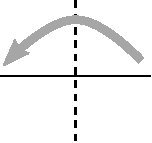
\includegraphics{../graphics/origamiBisect.pdf}
\]
\end{construction}

\begin{question} 
Which rule for folding and tracing constructions are we using above?
\end{question}
\QM


\begin{construction}[Perpendicular through a Point]\index{folding and tracing!perpendicular through a point}  
Given a point and a line, we wish to construct a line perpendicular to
the original line that passes through the given point.
\begin{enumerate}
\item Fold the given line onto itself so that the crease passes though
  the given point.
\item The crease will be the perpendicular line.
\end{enumerate}
\[
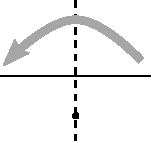
\includegraphics{../graphics/origamiPerpPoint.pdf}
\]
\end{construction}

\begin{question} Which rule for folding and tracing constructions are we using above?
\end{question}
\QM




\begin{construction}[Bisecting an Angle]\index{folding and tracing!bisecting an angle} 
We wish to divide an angle in half.
\begin{enumerate}
\item Fold a point on one leg of the angle to the other leg so that
  the crease passes though the vertex of the angle.
\item The crease will bisect the angle.
\end{enumerate}
\[
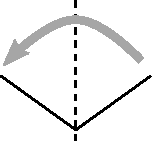
\includegraphics{../graphics/origamiBangle.pdf}
\]
\end{construction}


\begin{question} Which rule for folding and tracing constructions are we using above?
\end{question}
\QM



\begin{construction}[Parallel through a Point]\index{folding and tracing!parallel through a point} 
 Given a line and a point, we wish to construct another line parallel
 to the first that passes through the given point.
\begin{enumerate}
\item Fold a perpendicular line through the given point.
\item Fold a line perpendicular to this new line through the given
  point.
\end{enumerate}
\[
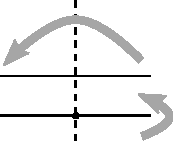
\includegraphics{../graphics/origamiParaPoint.pdf}
\]
\end{construction}



Now there may be a pressing question in your head:

\begin{question} 
How the heck are we going to fold a circle?
\end{question}

First of all, remember the definition of a circle:

\begin{definition}\index{circle}
A \textbf{circle} is the set of points that are a fixed distance from
a given point.
\end{definition}

\begin{question} Is the center of a circle part of the circle?
\end{question}
\QM

Secondly, remember that when doing compass and straightedge
constructions we can \textbf{only} mark points that are intersections
of lines and lines, lines and circles, and circles and circles. Thus
while we technically draw circles, we can only actually mark certain
points on circles.  When it comes to folding and tracing constructions, drawing a
circle amounts to marking points a given distance away from a given
point---that is exactly what we can do with compass and straightedge
constructions.


\begin{construction}[Intersection of a Line and a Circle]
\index{folding and tracing!intersection of a line and a circle} We wish to
construct the points where a given line meets a given circle. Note: A
circle is given by a point on the circle and the central point.
\begin{enumerate} 
\item Fold the point on the circle onto the given line so that the
  crease passes through the center of the circle.
\item Mark this point though both sheets of paper onto the line.
\end{enumerate}
\[
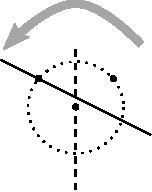
\includegraphics{../graphics/origamiCircLine.pdf}
\]
\end{construction}

\begin{question} Which rule for folding and tracing constructions are we using above?
\end{question}
\QM

\begin{question} How could you check that your folding and tracing construction is correct?
\end{question}
\QM

\begin{construction}[Equilateral Triangle]\index{folding and tracing!equilateral triangle} 
We wish to construct an equilateral triangle given the length of one
side.
\begin{enumerate} 
\item Bisect the segment.
\item Fold one end of the segment onto the bisector so that the crease
  passes through the other end of the segment. Mark this point onto
  the bisector.
\item Connect the points.
\end{enumerate}
\[
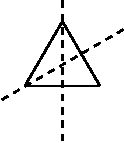
\includegraphics{../graphics/origamiTriangle.pdf}
\]
\end{construction}

\begin{question} Which rules for folding and tracing constructions are we using above?
\end{question}
\QM







\begin{construction}[Intersection of Two Circles]\index{folding and tracing!intersection of two circles} 
We with to intersect two circles, each given by a center point and a
point on the circle. 
\begin{enumerate}
\item Use four sheets of tracing paper. On the first sheet, mark the
  centers of both circles. On the next two sheets, mark the center and
  point on each of the circle---one circle per sheet. 
\item Simply move the two sheets with the centers and points on the
  circles, so that the centers are over the centers from the first
  sheet, and the points on the circles coincide. Now on the fourth
  sheet, mark all points.
\end{enumerate}
\end{construction}
\QM


Think about the definition of a circle. In a similar fashion we can
define other common geometric figures:


\begin{definition} 
Given a point and a line, a \textbf{parabola}\index{parabola} is the
set of points such that each of these points is the same distance from
the given point as it is from the given line.
\[
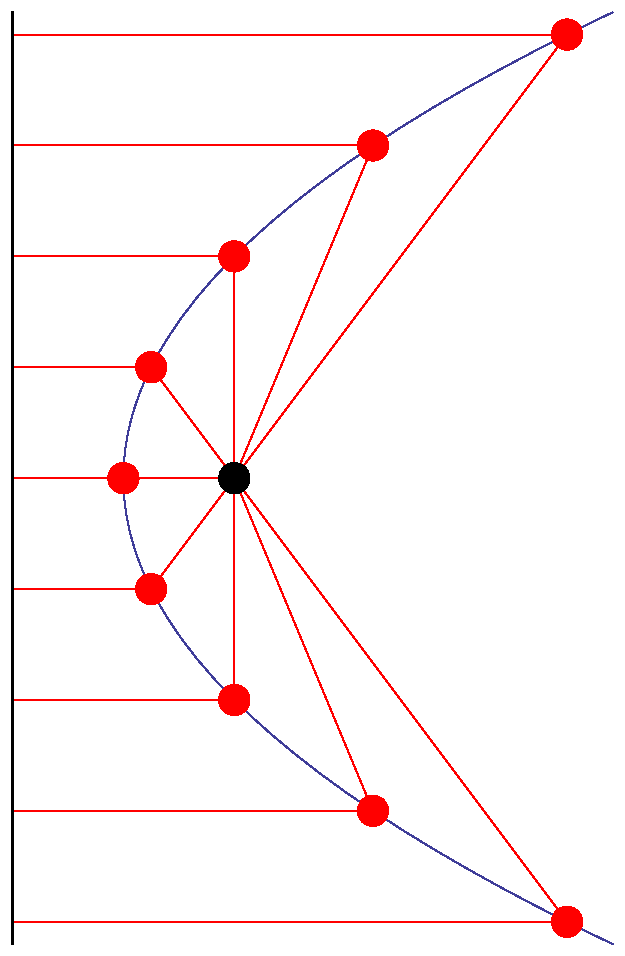
\includegraphics[angle=90,scale=.4]{../graphics/parabolapointline.pdf}
\]
\end{definition}

We can also form a parabola from an \textit{envelope of
  tangents}:\index{envelope of tangents}
\[
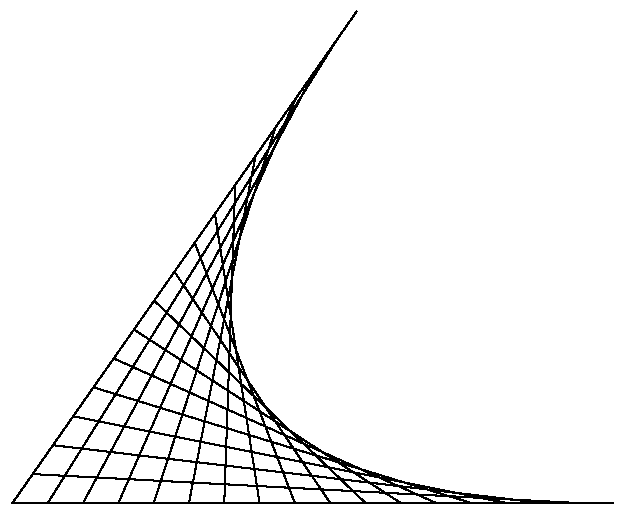
\includegraphics[scale=.6]{../graphics/envelope.pdf}
\]
Using a similar idea we can essentially obtain a parabola using
folding and tracing.

\begin{construction}[Parabola]\index{folding and tracing!parabola} 
Given a point and a line we wish to construct a parabola.
\begin{enumerate}
\item Make a series of equally spaced marks on your line. 
\item Fold the point onto the marks.
\item Repeat the above step until an envelope of tangents forms.
\end{enumerate}
\end{construction}

\begin{question} 
Considering the definition of the parabola, can you explain why the
above construction makes sense?
\end{question}
\QM

\begin{question} Can you give a compass and straightedge construction of a parabola?
\end{question}
\QM

Our final basic folding and tracing construction is one that \textbf{cannot} be
done with compass and straightedge alone.\marginnote{This construction was discovered by S.T.\ Gormsen and verified by S.H.\ Kung.}



\begin{construction}[Angle Trisection]\index{trisecting the angle}\index{folding and tracing!trisecting the angle}
We wish to divide an angle into thirds.
\begin{enumerate}
\item Bisect the given angle.
\item Find two points (one on each leg of the angle) equidistant from the vertex of the angle.
\item Fold the two points found above so that one of them lands on the
  extension (behind the angle) of the angle bisector and one lands on
  the line containing the other leg of the triangle---this will be
  behind the vertex. You are basically folding the angle back over
  itself.
\item The crease from the last step will intersect the angle bisector
  at some point, mark it.
\item The angle with the above mark as its vertex, the bisector found
  above as one of its legs, and the line to either of the points found
  in step 2 above will be one third of the starting angle.
\end{enumerate}
\[
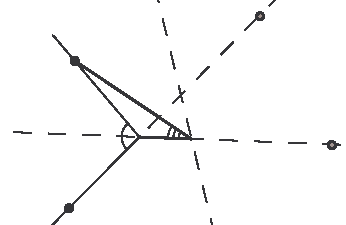
\includegraphics{../graphics/origamiTrisection.pdf}
\]
\end{construction}


\begin{problems}
\begin{enumerate}
\item What are the rules for folding and tracing constructions?
\item Use folding and tracing to bisect a given line segment. Explain the steps in
  your construction.
\item Given a line segment with a point on it, use folding and tracing to
  construct a line perpendicular to the segment that passes through
  the given point. Explain the steps in your construction.
\item Use folding and tracing to bisect a given angle. Explain the steps in your
  construction.
\item Given a point and line, use folding and tracing to construct a line parallel
  to the given line that passes through the given point. Explain the
  steps in your construction.
\item Given a point and line, use folding and tracing to construct a line
  perpendicular to the given line that passes through the given
  point. Explain the steps in your construction.
\item Given a circle (a center and a point on the circle) and line,
  use folding and tracing to construct the intersection. Explain the steps in your
  construction.
\item Given a line segment, use folding and tracing to construct an equilateral
  triangle whose edge has the length of the given segment. Explain the
  steps in your construction.
\item Explain how to use folding and tracing to transfer a segment.
\item Given an angle and some point, use folding and tracing to copy the angle so
  that the new angle has as its vertex the given point. Explain the
  steps in your construction.
\item Explain how to use folding and tracing to construct envelope of tangents for
  a parabola.
\item Explain how to use folding and tracing to trisect a given angle.
\item Use folding and tracing to construct a square. Explain the steps in your construction.
\item Use folding and tracing to construct a regular hexagon. Explain the steps in
  your construction.
\item Morley's Theorem states:\index{Morley's Theorem}
If you trisect the angles of any triangle with lines, then those lines
form a new equilateral triangle inside the original triangle.\index{equilateral triangle}\index{trisecting the angle}
\[
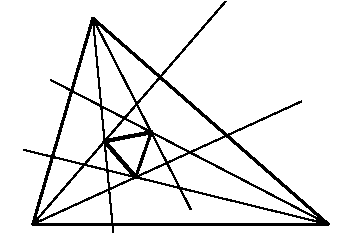
\includegraphics[scale=.5]{../graphics/morley.pdf}
\]
Give a folding and tracing construction illustrating Morley's Theorem. Explain the
steps in your construction.
\item Given a length of $1$, construct a triangle whose perimeter is a
  multiple of $6$. Explain the steps in your construction.
\item Construct a $30$-$60$-$90$ right triangle. Explain the steps in your
  construction.
\item Given a length of $1$, construct a triangle with a perimeter of
  $3 + \sqrt{5}$. Explain the steps in your construction.
\end{enumerate}
\end{problems}

\newpage


\section{Anatomy of Figures Redux}


Remember, in studying geometry we seek to discover the points that can
be obtained given a set of rules. Now the set of rules consists of the
rules for folding and tracing constructions.

\begin{question} 
In regards to folding and tracing constructions, what is a \textit{point}?
\end{question}
\QM

\begin{question}
In regards to folding and tracing constructions, what is a \textit{line}?
\end{question}
\QM


\begin{question}
In regards to folding and tracing constructions, what is a \textit{circle}?
\end{question}
\QM


OK, those are our basic figures, pretty easy right? Now I'm going to
quiz you about them (I know we've already gone over this, but it is
fundamental so just smile and answer the questions):

\begin{question} 
Place two points randomly in the plane. Do you expect to be able to
draw a single line that connects them?
\end{question}
\QM

\begin{question} 
Place three points randomly in the plane. Do you expect to be able to
draw a single line that connects them?
\end{question}
\QM

\begin{question} 
Place two lines randomly in the plane. How many points do you expect
them to share?
\end{question}
\QM


\begin{question} 
Place three lines randomly in the plane. How many points do you expect
all three lines to share?
\end{question}
\QM


\begin{question} 
Place three points randomly in the plane. Will you (almost!) always be
able to draw a circle containing these points? If no, why not? If yes,
how do you know?
\end{question}
\QM


%%%%%%%%%%%%%%%%%%%%%%%%%%%%%%%%%%%%%%%%%%%%%%%%%%%%%%%%%%%%%%%
%%%%%%%%%%%%%%%%%%%%%%%%%%%%%%%%%%%%%%%%%%%%%%%%%%%%%%%%%%%%%%%
%\subsection{Parallel Lines}
%
%When working with geometry in the plane we have the following fact:
%
%\begin{quote}
%Given a line and a point there is a unique line parallel to the first
%line that passes through the given point.
%\end{quote}
%
%If you recall the Construction of a Parallel through a Point, you
%might say that this fact is self-evident. The key word in the
%statement above is \textit{unique}. This means ``one and only.''
%
%HERE HERE HERE HERE HERE HERE
%
% HOW TO DO THIS JUSTICE???
% I was thinking to use ASA and Euclid's axioms - but is that 
% the right way to go? I'm just not sure - maybe I should see 
% what they do in the Missouri books.
%%%%%%%%%%%%%%%%%%%%%%%%%%%%%%%%%%%%%%%%%%%%%%%%%%%%%%%%%%%%%%%
%%%%%%%%%%%%%%%%%%%%%%%%%%%%%%%%%%%%%%%%%%%%%%%%%%%%%%%%%%%%%%%



\begin{problems}
\begin{enumerate}
\item In regards to folding and tracing constructions, what is a \textit{circle}?
  Compare and contrast this to a naive notion of a circle.
\item Explain how a perpendicular bisector is different from an
  altitude. Use folding and tracing to illustrate the difference.
\item Explain how a median different from an angle bisector.  Use
  folding and tracing to illustrate the difference.
\item Given a triangle, use folding and tracing to construct the
  circumcenter. Explain the steps in your
  construction.\index{circumcenter}
\item Given a triangle, use folding and tracing to construct the
  orthocenter. Explain the steps in your
  construction.\index{orthocenter}
\item Given a triangle, use folding and tracing to construct the incenter. Explain
  the steps in your construction.\index{incenter}
\item Given a triangle, use folding and tracing to construct the centroid. Explain
  the steps in your construction.\index{centroid}
\item Could the circumcenter be outside the triangle? If so explain
  how and use folding and tracing to give an example. If not, explain why not
  using folding and tracing to illustrate your ideas.
\item Could the orthocenter be outside the triangle? If so explain how and
  use folding and tracing to give an example. If not, explain why not using
  folding and tracing to illustrate your ideas.
\item Could the incenter be outside the triangle? If so explain how
  and use folding and tracing to give an example. If not, explain why not using
  folding and tracing to illustrate your ideas.
\item Could the centroid be outside the triangle? If so explain how
  and use folding and tracing to give an example. If not, explain why not using
  folding and tracing to illustrate your ideas.
\item Where is the circumcenter of a right triangle? Explain your
  reasoning and illustrate your ideas with folding and tracing.
\item Where is the orthocenter of a right triangle?  Explain your
  reasoning and illustrate your ideas with folding and tracing.


\item The following picture shows a triangle that has been folded
  along the dotted lines:
\[
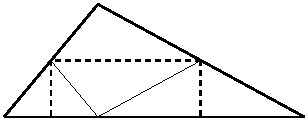
\includegraphics{../graphics/origamiPBPTri.pdf}
\]
Explain how the picture ``proves'' the following statements:
\begin{enumerate}
\item The interior angles of a triangle sum to $180^\circ$. 
\item The area of a triangle is given by $bh/2$. 
\end{enumerate}
\item Use folding and tracing to construct a triangle given the length of one
  side, the length of the the median to that side, and the length of
  the altitude of the opposite angle. Explain the steps in your
  construction.
\item Use folding and tracing to construct a triangle given one angle, the length
  of an adjacent side and the altitude to that side. Explain the steps
  in your construction.
\item Use folding and tracing to construct a triangle given one angle and the
  altitudes to the other two angles. Explain the steps in your
  construction.
\item Use folding and tracing to construct a triangle given two sides and the
  altitude to the third side. Explain the steps in your construction.
\end{enumerate}
\end{problems}


